\chapter{Moving Solitons in the Lugiato-Lefever equation.}

In section~\ref{sec:fra_LS} we introduced the concept of dissipative localized structures (LSs). Here, we will study the formation
of such structures in nonlinear optical systems where they are often called optical or cavity solitons. 
More specifically, we will analyze the paradigmatic Lugiato-Lefever equation (LLE) \cite{lugiatolefever1987} used to describe fiber resonators, and
study the formation of LSs when a fourth-order derivative and a non-local term are considered.


\section{Lugiato-Lefever equation.}

In 1987, Lugiato and Lefever proposed a simple yet extremely rich nonlinear partial differential equation to study the formation of patterns and localized states
in the framework of nonlinear optics \cite{lugiatolefever1987}. They considered a cavity filled with a nonlinear medium in the low transmission (or high quality) limit
driven by a continuous wave. In order to keep the equation as simple as possible, they considered a cubic nonlinearity which is characteristic of Kerr media. Moreover,
In virtue of the low dissipation limit, they originally neglected the longitudinal variable $z$ (along which light propagates) and kept only the transversal plane $x-y$ as spatial
variables in the equation. In contrast, a longitudinal (or temporal) LLE was later formulated by Haelterman and his colleagues [ref], where only the longitudinal 
coordinate becomes relevant. The main difference between these two equations is that in the former, a transversal Laplacian appears due to diffraction of the light, whereas
in the latter, a longitudinal Laplacian appears due to dispersion of the light. However, from a mathematical point of view, they are the same equations.


\begin{equation}
    \dfrac{\partial E}{\partial t} = E_{in} - (1 + i\theta) E + i |E|^2 E + i\nabla^2 E
    \label{lle:lle}
\end{equation}

In our case, we will consider the longitudinal LLE corresponding to Eq.~(\ref{lle:lle}) as a starting point and we will analyze
the effect of adding a fourth-order dispersion term and the Raman effect which will be explained in the following section.¿
Indeed, the dispersion curve can be highly controlled using photonic crystal fibers and, when operating
close to the zero dispersion wavelength, higher-order dispersion must be taken into account.

\section{Raman effect.}

Raman effect frequently observed 26-31. 

Stabilization of LSs by means of the Raman effect. 39, 41, 41-43 in normal dispersion and far from MI. 

\section{Isolas and traveling solitons.}

We will consider in the following sections a ring resonator operating close to the zero dispersion wavelength and pumped
with short pulses. Therefore, higher-order dispersion terms must be included along with the stimulated
Raman scattering. Taking into account these terms, the slowly varying envelope of the electric field within the
resonator is described by the following generalized Lugiato-Lefever equation.

\begin{equation}
    \dfrac{\partial E}{\partial \zeta} = E_i - (1 + i\Delta)E + i(1 - f_r)|E|^2 E 
                            + i \beta_2 \dfrac{\partial^2 E}{\partial T^2} + i \beta_4 \dfrac{\partial^4 E}{\partial T^4}
                            + i f_r E \int_{-\infty}^T \phi(T-T') |E(T')|^2 dT'
    \label{lle:glle}
\end{equation}             

Here, $E = E(\zeta, T)$ is the normalized mean-field cavity electric field, $E_i$ is the amplitude of the pumping field,
$Delta$ is the detuning between the pump frequency and that of the cavity, and losses are normalized to unity. The time $\zeta$ represents the
slow time scale along consecutive round trips and $T$ represents the fast time scale in the frame of reference
moving with the group velocity of the light within the resonator. The parameters $\beta_2$ and $\beta_4$ correspond to the
second and fourth-order dispersion, respectively. Lastly, the Raman-Kerr effect appears as the cubic local and non-local term,
characterized by the strength fraction of the Raman effect $f_r$ and the kernel function,

\begin{equation}
    \phi(T) = a \exp (-T / \tau_2) \sin (T / \tau_1)
    \label{lle:kernel}
\end{equation}

with $a = \tau_0 (\tau_1 ^2 + \tau_2 ^2)/(\tau_1 \tau_2 ^2)$. Typical values of these parameters for fused-silica-based fibers
[48 from 164] are $f_r = 0.18$, $\tau_1 = 12.2$ fs, and $\tau_2 = 32$ fs.

Close to the nascent optical bistability a Swift-Hohenberg equation with an additional nonlocal term due to the Raman effect
can be deduced for the deviation $u$ of the electric field from its value at the onset of the bistability.

\begin{equation}
    \partial_t u = \eta + \mu u - u^3 + \beta \partial_\tau^2 u - \partial_\tau^4 u + \int_{-\infty}^\tau \phi(\tau - \tau')u(\tau')d\tau'
    \label{lle:shraman}
\end{equation}

Note that for the numerical computation of the nonlocal term corresponding to the SRS we will exploit 

In that case the LS is formed due to front locking between the two CW solutions (i.e. it requires bistability). 
However, in this case the LS arise due to coexistence between periodic state and CW, so even in the monostable can be observed.


\begin{SCfigure}
    \centering
    \caption{Moving bright soliton obtained by numerical simulation of Eq.~(\ref{lle:lle}). Panel
    (a) shows the temporal evolution in both the slow ($\zeta$) and fast ($T$) time scales. Panels
    (b) and (c) show the temporal profile for $\zeta=0$ and Fourier spectrum, respectively. Parameters are
    $\Delta=1.7$, $E_{in}=1.219$, $f_r = 0.05$, $\beta_2 = 1$, $\beta_4 = 0.01$, $\tau_0=1$, $\tau_1=3$,
    $\tau_2=10$, $N=512$, $\Delta x=0.25$ and $\Delta t=0.001$.}
    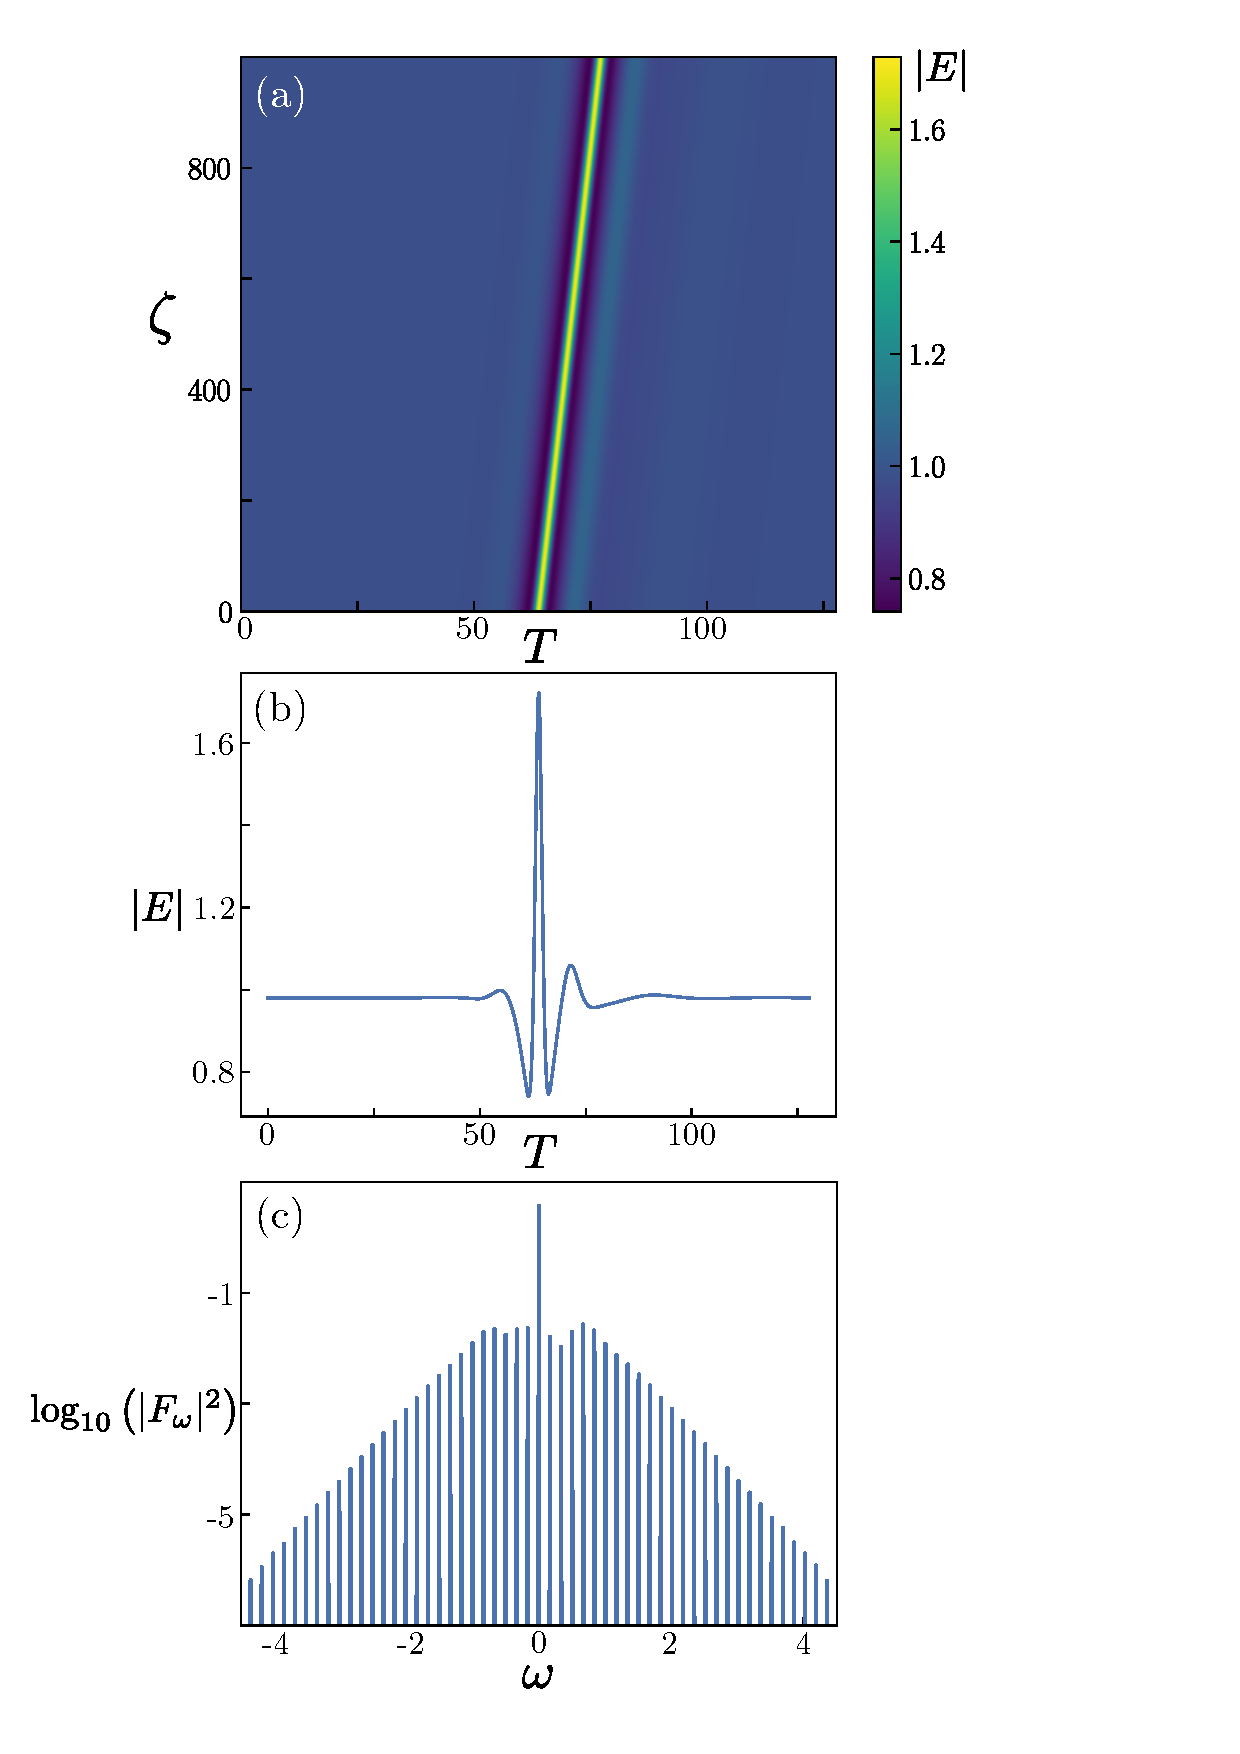
\includegraphics[width=0.6\textwidth]{imagenes/lle/LLE_Spatiotemporal.pdf}
\end{SCfigure}

\begin{figure}
    \centering
    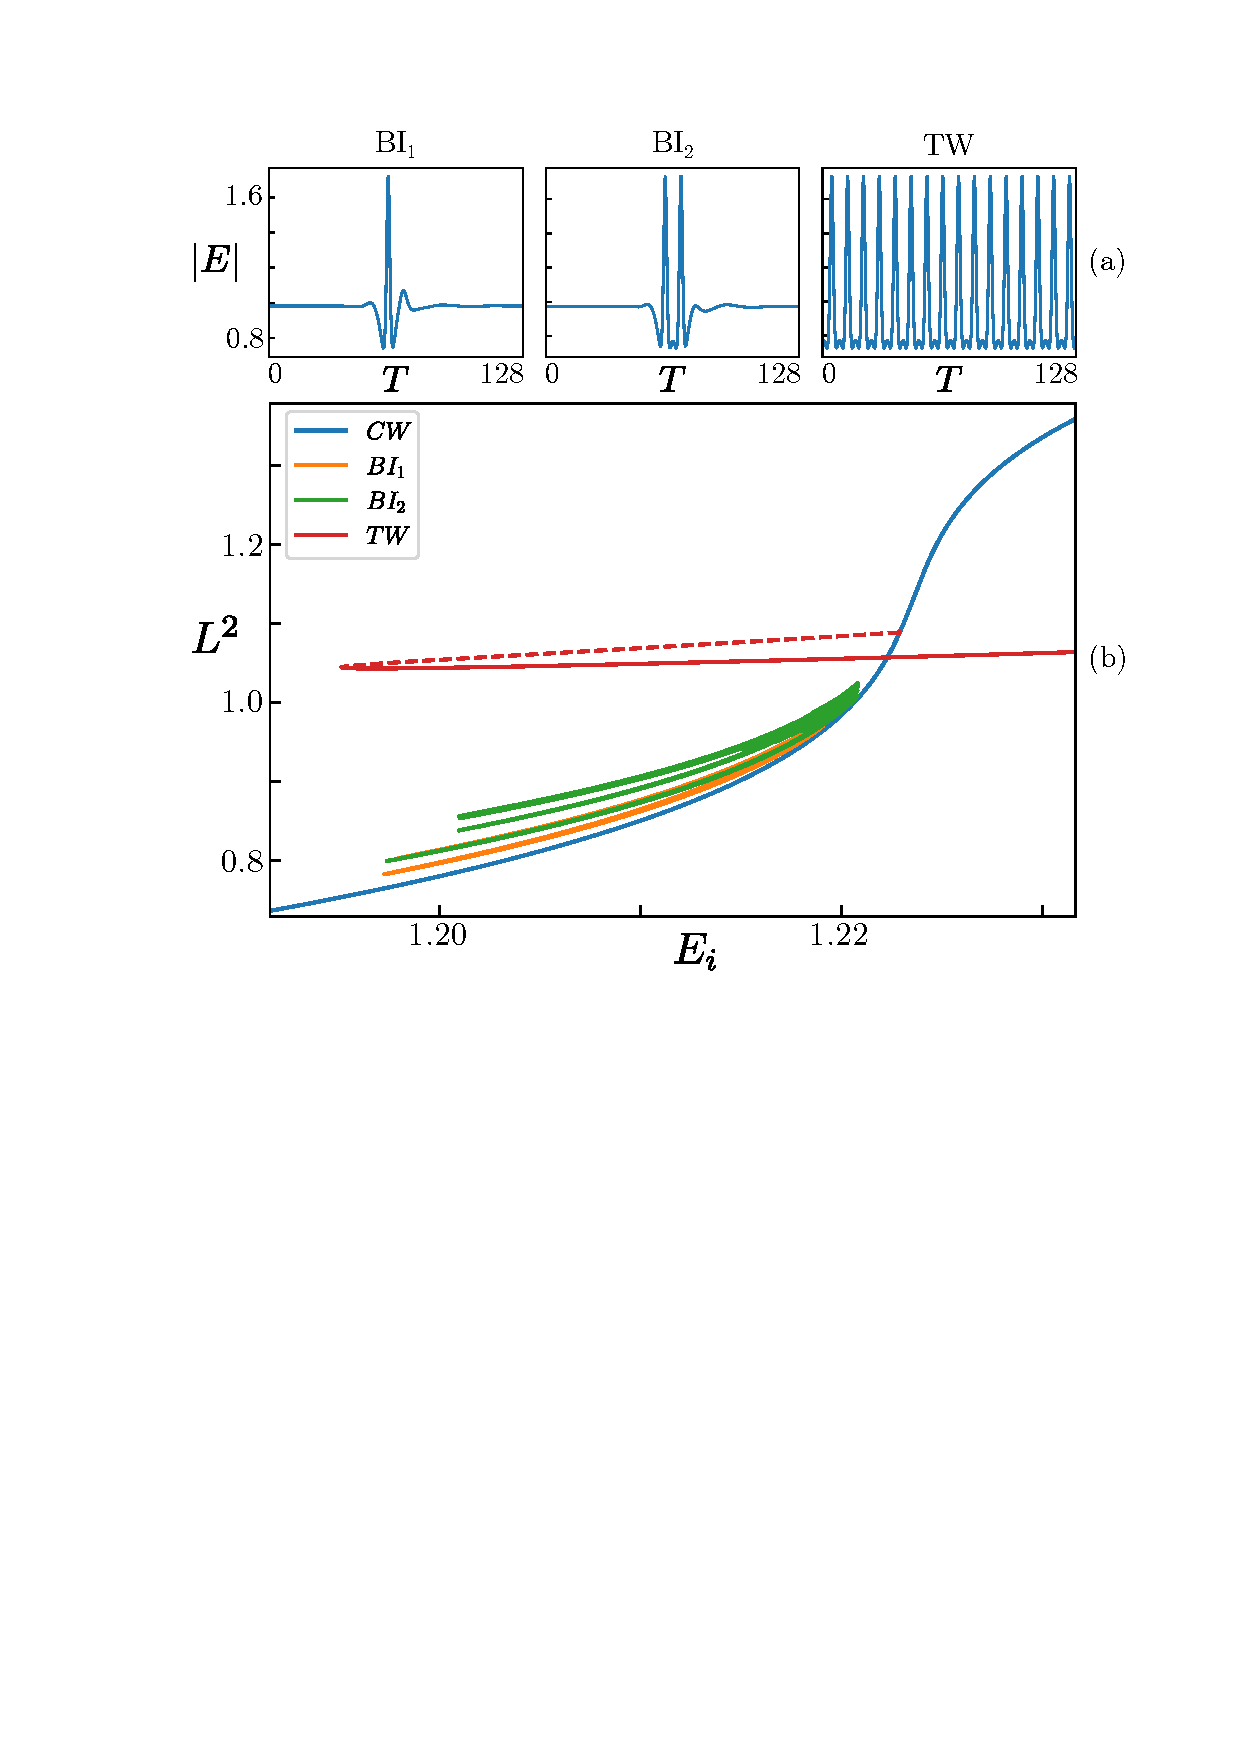
\includegraphics[width=0.7\textwidth]{imagenes/lle/LLE_Isola.pdf}
    \caption{asd}
\end{figure}

\section{A reduced model.}

\begin{SCfigure}
    \centering
    \caption{asdasd}
    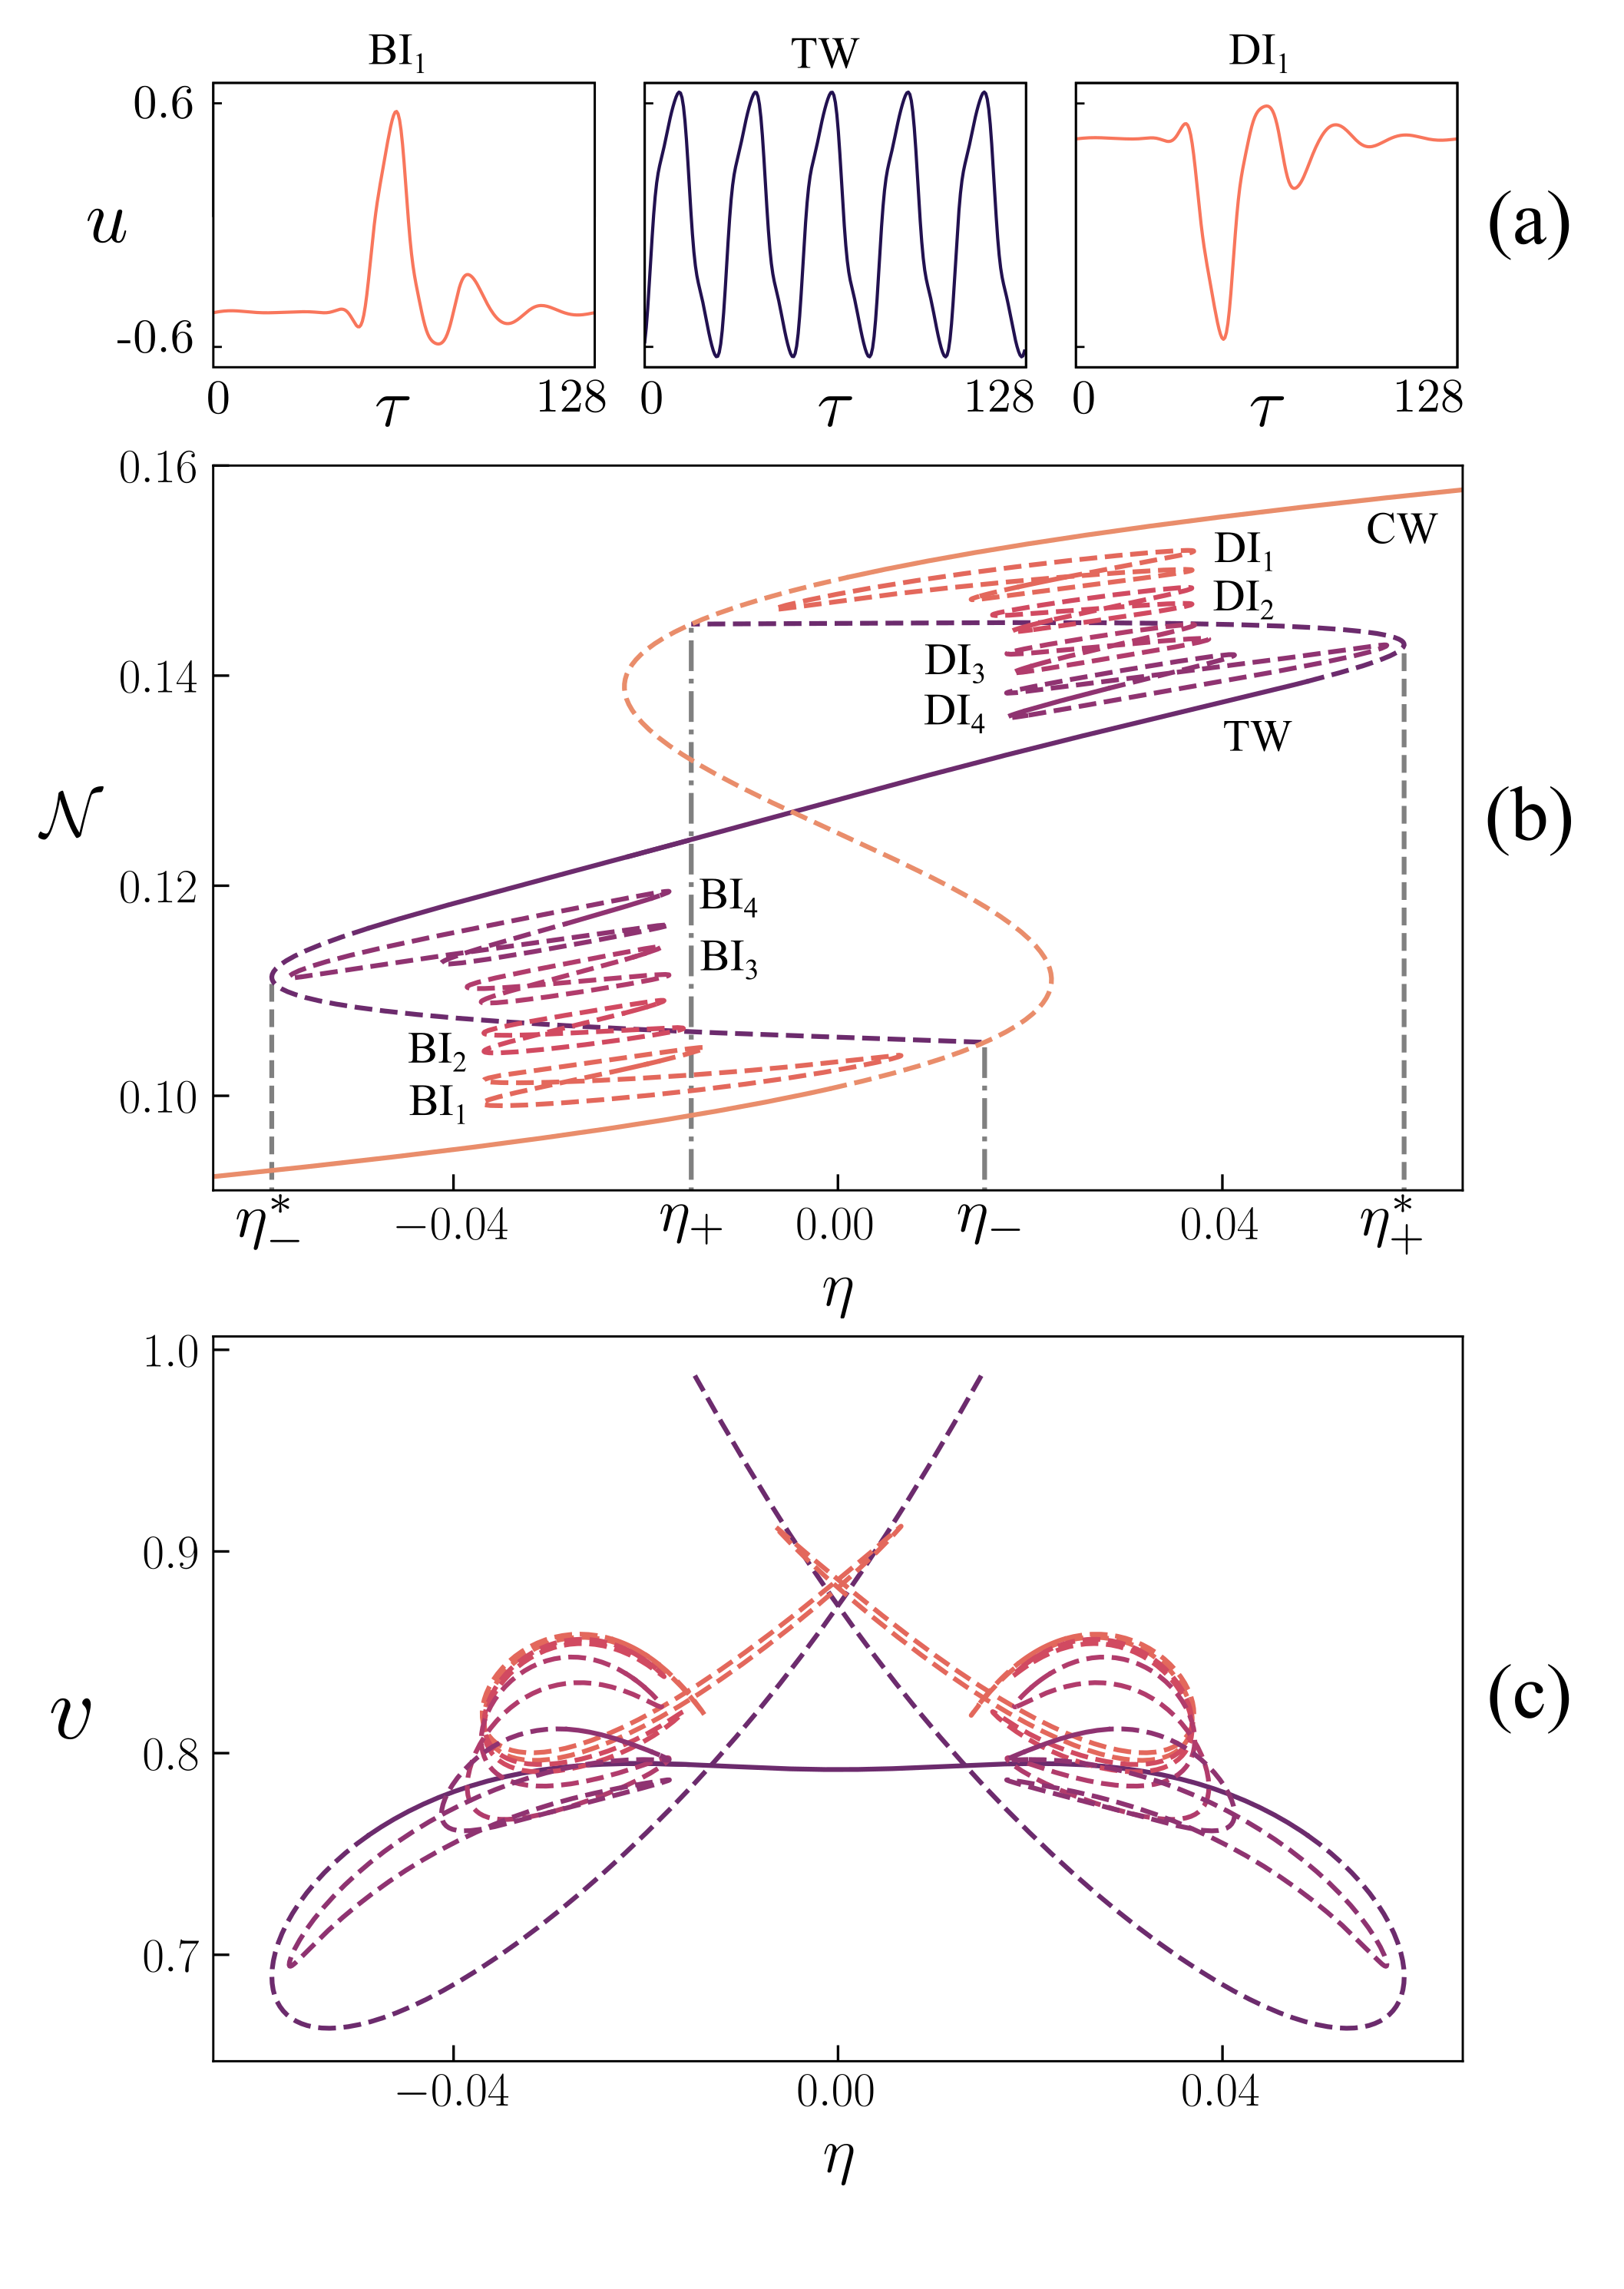
\includegraphics[width=0.6\textwidth]{imagenes/lle/Fig3.png}
\end{SCfigure}

\begin{figure}[h]
    \centering
    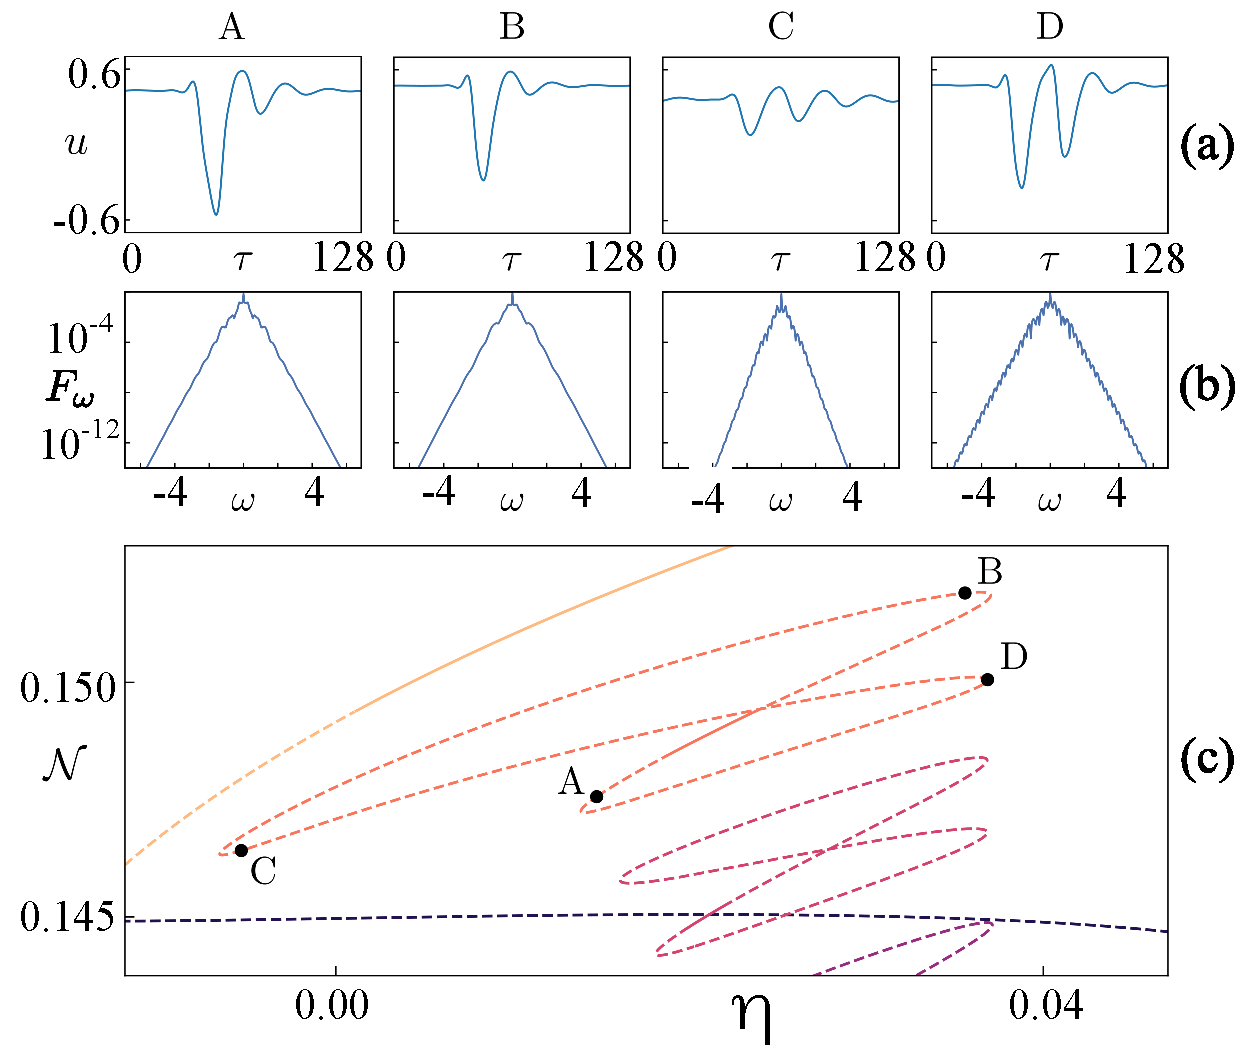
\includegraphics[width=0.5\textwidth]{imagenes/lle/Fig4-Isola.pdf}
    \caption{asd}
\end{figure}

\section{Oscillatory bound states.}

\begin{enumerate}
    \item 
\end{enumerate}